\documentclass[runningheads]{../../../llncs}
\usepackage[paperheight=295mm,paperwidth=210mm]{geometry}
\usepackage{graphicx}
\usepackage{import}
\usepackage{kotex}
\usepackage[dvipsnames]{xcolor}
\usepackage{fancyvrb}
\usepackage{listings}
\usepackage{indentfirst}
\usepackage{tabularx}
\usepackage{underscore}
\usepackage{multicol}
\usepackage{enumitem}
\usepackage{menukeys}
\usepackage{amsmath}
\usepackage{clrscode3e} % https://www.ctan.org/pkg/clrscode3e?lang=en
\usepackage[numbers,square,super]{natbib}
\usepackage{inconsolata} % Inconsolata
\usepackage{mathptmx} % Times New Roman
\usepackage{minted}
\graphicspath{ {./images/} }
\lstset{basicstyle=\footnotesize\ttfamily,breaklines=true}
\renewcommand{\bibname}{참고문헌}
\setlength{\parindent}{1em}
\setlength{\parskip}{1em}
\linespread{1.2}
{\renewcommand{\arraystretch}{1.5}%
\setlength{\tabcolsep}{0.5em}%
\newenvironment{Figure}
  {\par\medskip\noindent\minipage{\linewidth}}
  {\endminipage\par\medskip}
\newcommand{\translation}[1]{\textsuperscript{#1}}
\newlist{algorithm}{enumerate}{10}
\setlist[algorithm]{label*=\arabic*.}
\setlist[algorithm,1]{label=\textbf{\arabic*}}
\setlist[algorithm,2]{label=\textbf{\alph*}}
\setlist[algorithm,3]{label=\textbf{\roman*}}
\setlist[algorithm,4]{label=(\arabic*)}
\setlist[algorithm,5]{label=(\alph*)}
\setlist[algorithm,6]{label=(\roman*)}
\makeatletter
\renewcommand\NAT@citesuper[3]{\ifNAT@swa
\if*#2*\else#2\NAT@spacechar\fi
\unskip\kern\p@\textsuperscript{\NAT@@open#1\if*#3*\else,\NAT@spacechar#3\fi\NAT@@close}%
   \else #1\fi\endgroup}
\makeatother
	
\begin{document}

\title{CSE3013 (컴퓨터공학 설계 및 실험 I) \space \newline WEB-1 예비 보고서}
\author{서강대학교 컴퓨터공학과 박수현 (20181634)}
\institute{서강대학교 컴퓨터공학과}
\maketitle

\section{목적}
실험 내용의 기초가 되는 HTML 문법을 미리 숙지하여 본 실험에 임할 수 있도록 한다.

\section{예비 학습}

\subsection{문자 및 조판}

\begin{multicols}{2}
	\begin{Figure}
		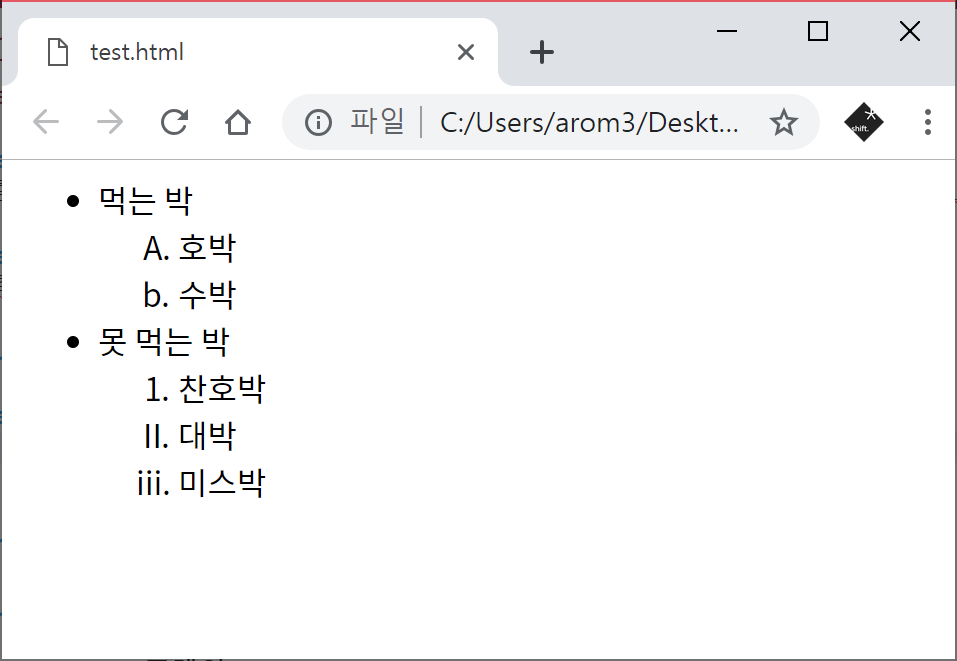
\includegraphics[width=\linewidth]{preview-2-1}
		\label{fig:preview-2-1}
	\end{Figure}
	\columnbreak
	\inputminted[xleftmargin=\parindent,linenos]{html}{inc-sources/source-2-1.html}
\end{multicols}

\subsection{테이블}

\begin{multicols}{2}
	\begin{Figure}
		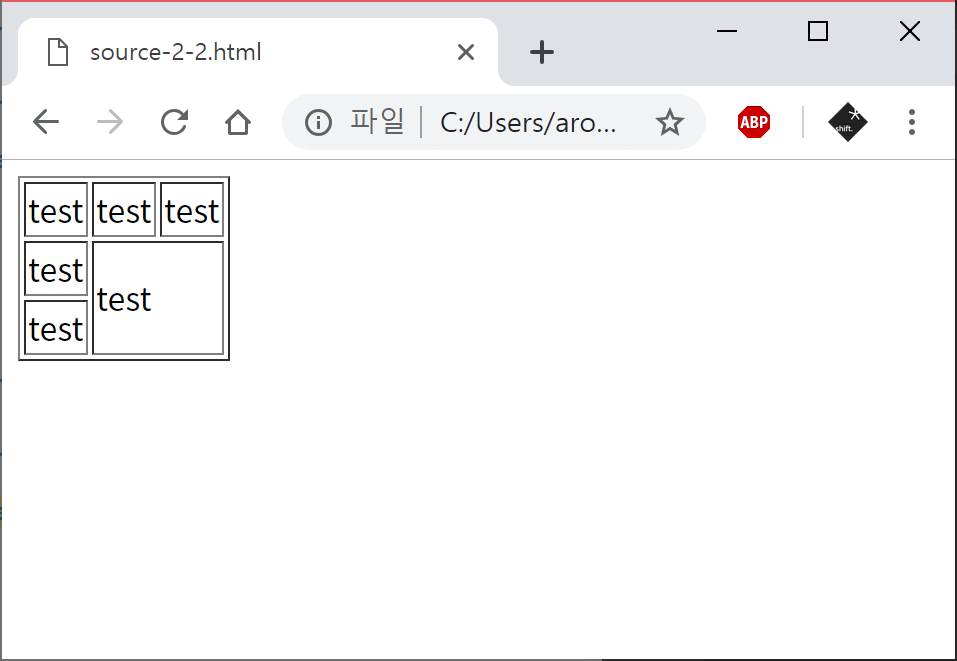
\includegraphics[width=\linewidth]{preview-2-2}
		\label{fig:preview-2-2}
	\end{Figure}
	\columnbreak
	\inputminted[xleftmargin=\parindent,linenos]{html}{inc-sources/source-2-2.html}
\end{multicols}

\subsection{프레임}

\begin{multicols}{2}
	\begin{Figure}
		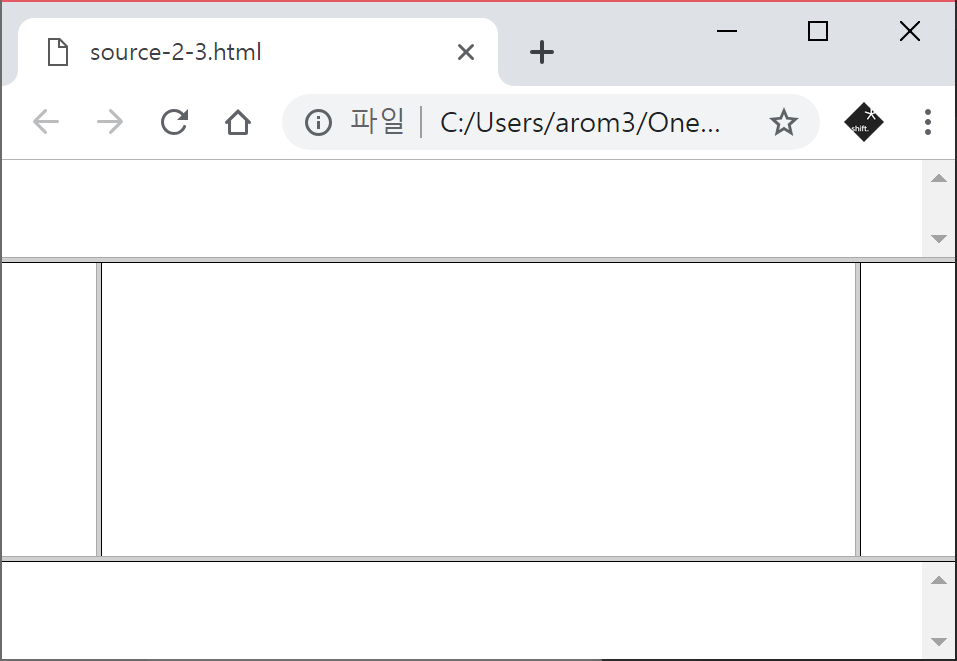
\includegraphics[width=\linewidth]{preview-2-3}
		\label{fig:preview-2-3}
	\end{Figure}
	\columnbreak
	\inputminted[xleftmargin=\parindent,linenos]{html}{inc-sources/source-2-3.html}
\end{multicols}

\section{보충 학습}

HTML, CSS, JavaScript는 현대 웹을 이루는 대표적인 기술들이다. HTML(Hypertext Markup Language)은 웹 사이트의 구조를 정의하는 마크업 언어이고, CSS(Cascading Stylesheet)는 웹 사이트의 외관을 정의하는 스타일시트이다. JavaScript는 스크립트 언어로 그 사용이 웹에 국한되어 있지는 않으나, 웹에서는 유저와의 상호작용, 애니메이션, 서버와의 통신 등 다양한 일을 담당한다.

\textbf{브라우저 엔진}은 이 파일들을 사용자가 읽을 수 있는 형태로 렌더해 주는 프로그램을 일컫는다. Firefox와 Opera 브라우저가 사용하는 \textbf{Gecko}, Chrome이나 Safari 등의 브라우저가 사용하는 \textbf{WebKit}, 그리고 지금은 지원이 종료된 Internet Explorer가 사용하는 \textbf{Trident} 등이 대표적 브라우저 엔진이다.

같은 웹 사이트라면 어떤 사용자에게나 같은 화면을 보여주는 것이 이상적이겠지만, 브라우저 엔진마다 HTML, CSS, JS 각각을 해석하는 방법이 조금씩 다르다. 이런 이유로 엔진마다 사용자에게 렌더되는 내용을 일관적으로 보이게 하기 위해 만들어진 것이 웹 언어 \textbf{표준}이다. HTML과 CSS는 \textbf{W3C}(World Wide Web Consortium)에 의해 표준화되어 있고, JavaScript는 ECMA International의 \textbf{ECMAScript} 표준을 따른다. 브라우저 엔진들은 이 표준에 명세되어 있는 항목들을 구현해야 한다.

최근 들어 특히 외국 사이트에서 Internet Explorer에서만 정상적으로 표시되지 않는 사이트들을 종종 볼 수 있게 되었다. 이는 IE와 IE의 엔진인 Trident에 대한 개발사 Microsoft의 지원이 종료되면서, IE가 더 이상 최신 표준을 지원하지 않게 되었기 때문이다. 현대 브라우저 엔진들인 Gecko와 WebKit은 HTML5, CSS3, ECMAScript 6 (ES6) 표준을 대부분 지키도록 구현되어 있으나 Trident는 HTML 4.01과 ES5 정도만 구현되어 있는 상태로 머물러 있다.

브라우저 엔진마다 갖고 있는 \textbf{독자 표준}도 있고, 독자 표준이 실제 표준이 되는 경우도 있다. 가령 CSS에서 요소의 변환을 의미하는 속성 \texttt{transform}은 W3C에 의해 표준으로 인정되기 전에 WebKit 등 일부 엔진에서만 \texttt{-webkit-transform}과 같은 형태로 사용할 수 있었다. 또한 현재 요소 뒤에 있는 모든 요소에 필터를 적용하는 \texttt{-webkit-backdrop-filter}와 같은 속성도 있다. WebKit은 Apple의 주도로 개발되고 있는데, \texttt{-webkit-backdrop-filter}로 뒤의 요소들에 전부 \texttt{blur()} 효과를 주면 Apple의 대표 운영체제 macOS의 디자인 패턴을 쉽게 구현할 수 있기 때문이라고 추측된다. 현재 \texttt{-webkit-backdrop-filter}는 W3C Filter Effects Module Level 2 표준으로 제안되어 있다.

\begin{minted}{html}

\end{minted}
  
\end{document}
